% Format:  Latex Orientation:  Portrait
% MASTERFILE
%
% Last change: <Thu, 2016/05/26 10:25:26 arwagner l00slwagner.desy.de>
%
\documentclass[presentation, 10pt]{beamer}
% use ``handout'' instead of ``presentation'' to create a 2 on 1 page
% handout version of the document

\mode<handout>{%
	\usepackage{pgf}
	\usepackage{pgfpages}
	\pgfpagesuselayout{2 on 1}[a4paper,border shrink=5mm]
}
\mode<presentation>{%
	\usetheme{DESY}
}
%% Setup for Beamer
\usepackage{xcolor}
\usepackage{hyperxmp}
% \usepackage[pdfa]{hyperref}
\usepackage{luatextra}
\usepackage{wasysym}
\usepackage{eurosym}
\usepackage{bookmark}
\usepackage{graphicx}
\usepackage{fontspec}
\setmainfont{Arial}
\usepackage[ngerman,english]{babel}
\usepackage{xspace}
\usepackage{tikz}

\tikzset{%
  every overlay node/.style={%
    %draw=black,fill=white,rounded corners,anchor=north west,
    draw=fzjlightblue,fill=fzjgray30,rounded corners,anchor=north west,
  },
}
% Usage:
% \tikzoverlay at (-1cm,-5cm) {content};
% or
% \tikzoverlay[text width=5cm] at (-1cm,-5cm) {content};
\def\tikzoverlay{%
   \tikz[baseline,overlay]\node[every overlay node]
}%


% General new commands an macros
\renewcommand{\emph}[1]{\structure{#1}}

\newcommand{\link}[2]{\href{#1}{~#2}}

\newcommand{\jointwo}{\textbf{JOIN$^2$}\xspace}

\newcommand{\BibTeX}{Bib\TeX}
\newcommand{\JabRef}{\link{http://jabref.sf.net}{JabRef}\xspace}
\newcommand{\Companion}[1]{\textit{\link{http://julib.fz-juelich.de/uhtbin/field-search-sort/001/PBYR/213964}{\LaTeX{} Companion}, #1}\xspace}
\newcommand{\pkg}[1]{\emph{\texttt{#1}}\xspace}

% general colour definitions
\newcommand{\smallgray}[1]{{\tiny\emph{#1}}}

\newcommand{\idR}{i.~d.~R.\xspace}
\newcommand{\va}{v.~a.\xspace}
\newcommand{\sa}{s.~a.\xspace}
\newcommand{\zB}{z.~B.\xspace}
\newcommand{\zT}{z.~T.\xspace}
\newcommand{\ggf}{ggf.\xspace}
\newcommand{\eg}{e.~g.\xspace}

\newcommand{\bs}[1]{\texttt{$\backslash$#1}}
\newcommand{\command}[2]{\texttt{\bs{#1}\{#2\}}}
% http://tex.stackexchange.com/questions/16447/beamer-top-aligning-columns-within-a-top-aligned-fram
\makeatletter
\newenvironment{topitemize}{%
   \setlength{\topsep}{0pt}
   \setlength{\partopsep}{0pt}
   \renewcommand*{\@listi}{\leftmargin\leftmargini \parsep\z@ \topsep\z@ \itemsep\z@}
   \let\@listI\@listi
   \itemize
}{\enditemize}
\makeatother


\title{DQM4HEP \\ Status and prospects}
% subtitle is required for DESY beamer, set at least a space ~
\subtitle{CHEF 2017 - Lyon}

\author[R. Ete]{\underline{R. Ete}, A. Pingault, T. Coates}
\institute{DESY}
\date{\today}

\newenvironment{topitemize}{%
   \setlength{\topsep}{0pt}
   \setlength{\partopsep}{0pt}
   \renewcommand*{\@listi}{\leftmargin\leftmargini \parsep\z@ \topsep\z@ \itemsep\z@}
   \let\@listI\@listi
   \itemize
}{\enditemize}

\usepackage{makecell}

%---------------------------------------------------------------------

\begin{document}

\maketitle

%----------------------------------------------------------------------
\begin{frame}
  \frametitle{Summary}

  \begin{itemize}
    \item Introduction
    \item Framework presentation
    \item Experiments running with DQM4HEP
    \item EUDAQ / DQM4HEP interface
    \item Current status
    \item Ongoing and future work
  \end{itemize}
  
\end{frame}

%----------------------------------------------------------------------
\begin{frame}
  \frametitle{Introduction}
  \footnotesize
  DQM systems in HEP domain :
  \begin{itemize}
    \item Evaluate data quality and alert users of anomalies
    \item Yet developed for most of HEP experiments (i.e AMORE or CMSSW)
    \item Provide for online and offline analysis
    \begin{itemize}
      \item Automatic data quality tests, possibly with reference histograms
      \item Distributed system for online analysis (data collectors)
      \item Dedicated visualization interface (Qt, Web)
    \end{itemize}
  \end{itemize}
  ~\\
  \textbf{But ...} Based on experiment specific event format
  \begin{itemize}
    \item Not re-usable by other experiments
    \item Duplicated software
    \item Ad-hoc solution for test-beam setup monitoring
  \end{itemize}
  ~\\
  Development of a generic DQM software for any HEP experiment : \textbf{DQM4HEP}
\end{frame}



%----------------------------------------------------------------------
\begin{frame}
  \frametitle{DQM4HEP}
  \framesubtitle{Software overview}
  \footnotesize
  Key points : 
  \begin{itemize}
    \item Standalone plugin system (dynamic shared lib loading) 
    \item \textbf{Event data model/format + event streaming abstraction}
  \end{itemize}
  ~ \\
  More general features :
  \begin{itemize}
    \item Online analysis (API)
    \item Streaming tools for event read/write functions
    \item Distributed system (DIM)
    \item Data collectors : event and histogram collector servers
    \item Quality test tools : interface + many templates
  \end{itemize}
\end{frame}


%----------------------------------------------------------------------
\begin{frame}
  \frametitle{DQM4HEP}
  \framesubtitle{Quality test API}
  \footnotesize
  \begin{block}{Monitor element}
    \begin{itemize}
      \item Wrap a ROOT TObject 
      \item Optional hold a ROOT TObject as reference
    \end{itemize}
  \end{block}
  \begin{block}{Quality test}
    \begin{itemize}
      \item Implement the logic a testing a monitor element
      \item Output a quality report (quality flag, success, etc)
    \end{itemize}
  \end{block}
  One monitor element can be tested with many QTests, i.e : \\
  \begin{itemize}
    \item Kolmogorov test using a reference histogram
    \item Mean of histogram within an expected value
  \end{itemize}
  One QTest can be attached to many monitor elements, i.e :
  \begin{itemize}
    \item Test different histograms with expected same gaussian distribution parameters
  \end{itemize}
\end{frame}


%----------------------------------------------------------------------
\begin{frame}
  \frametitle{DQM4HEP}
  \framesubtitle{Online architecture}
  \centering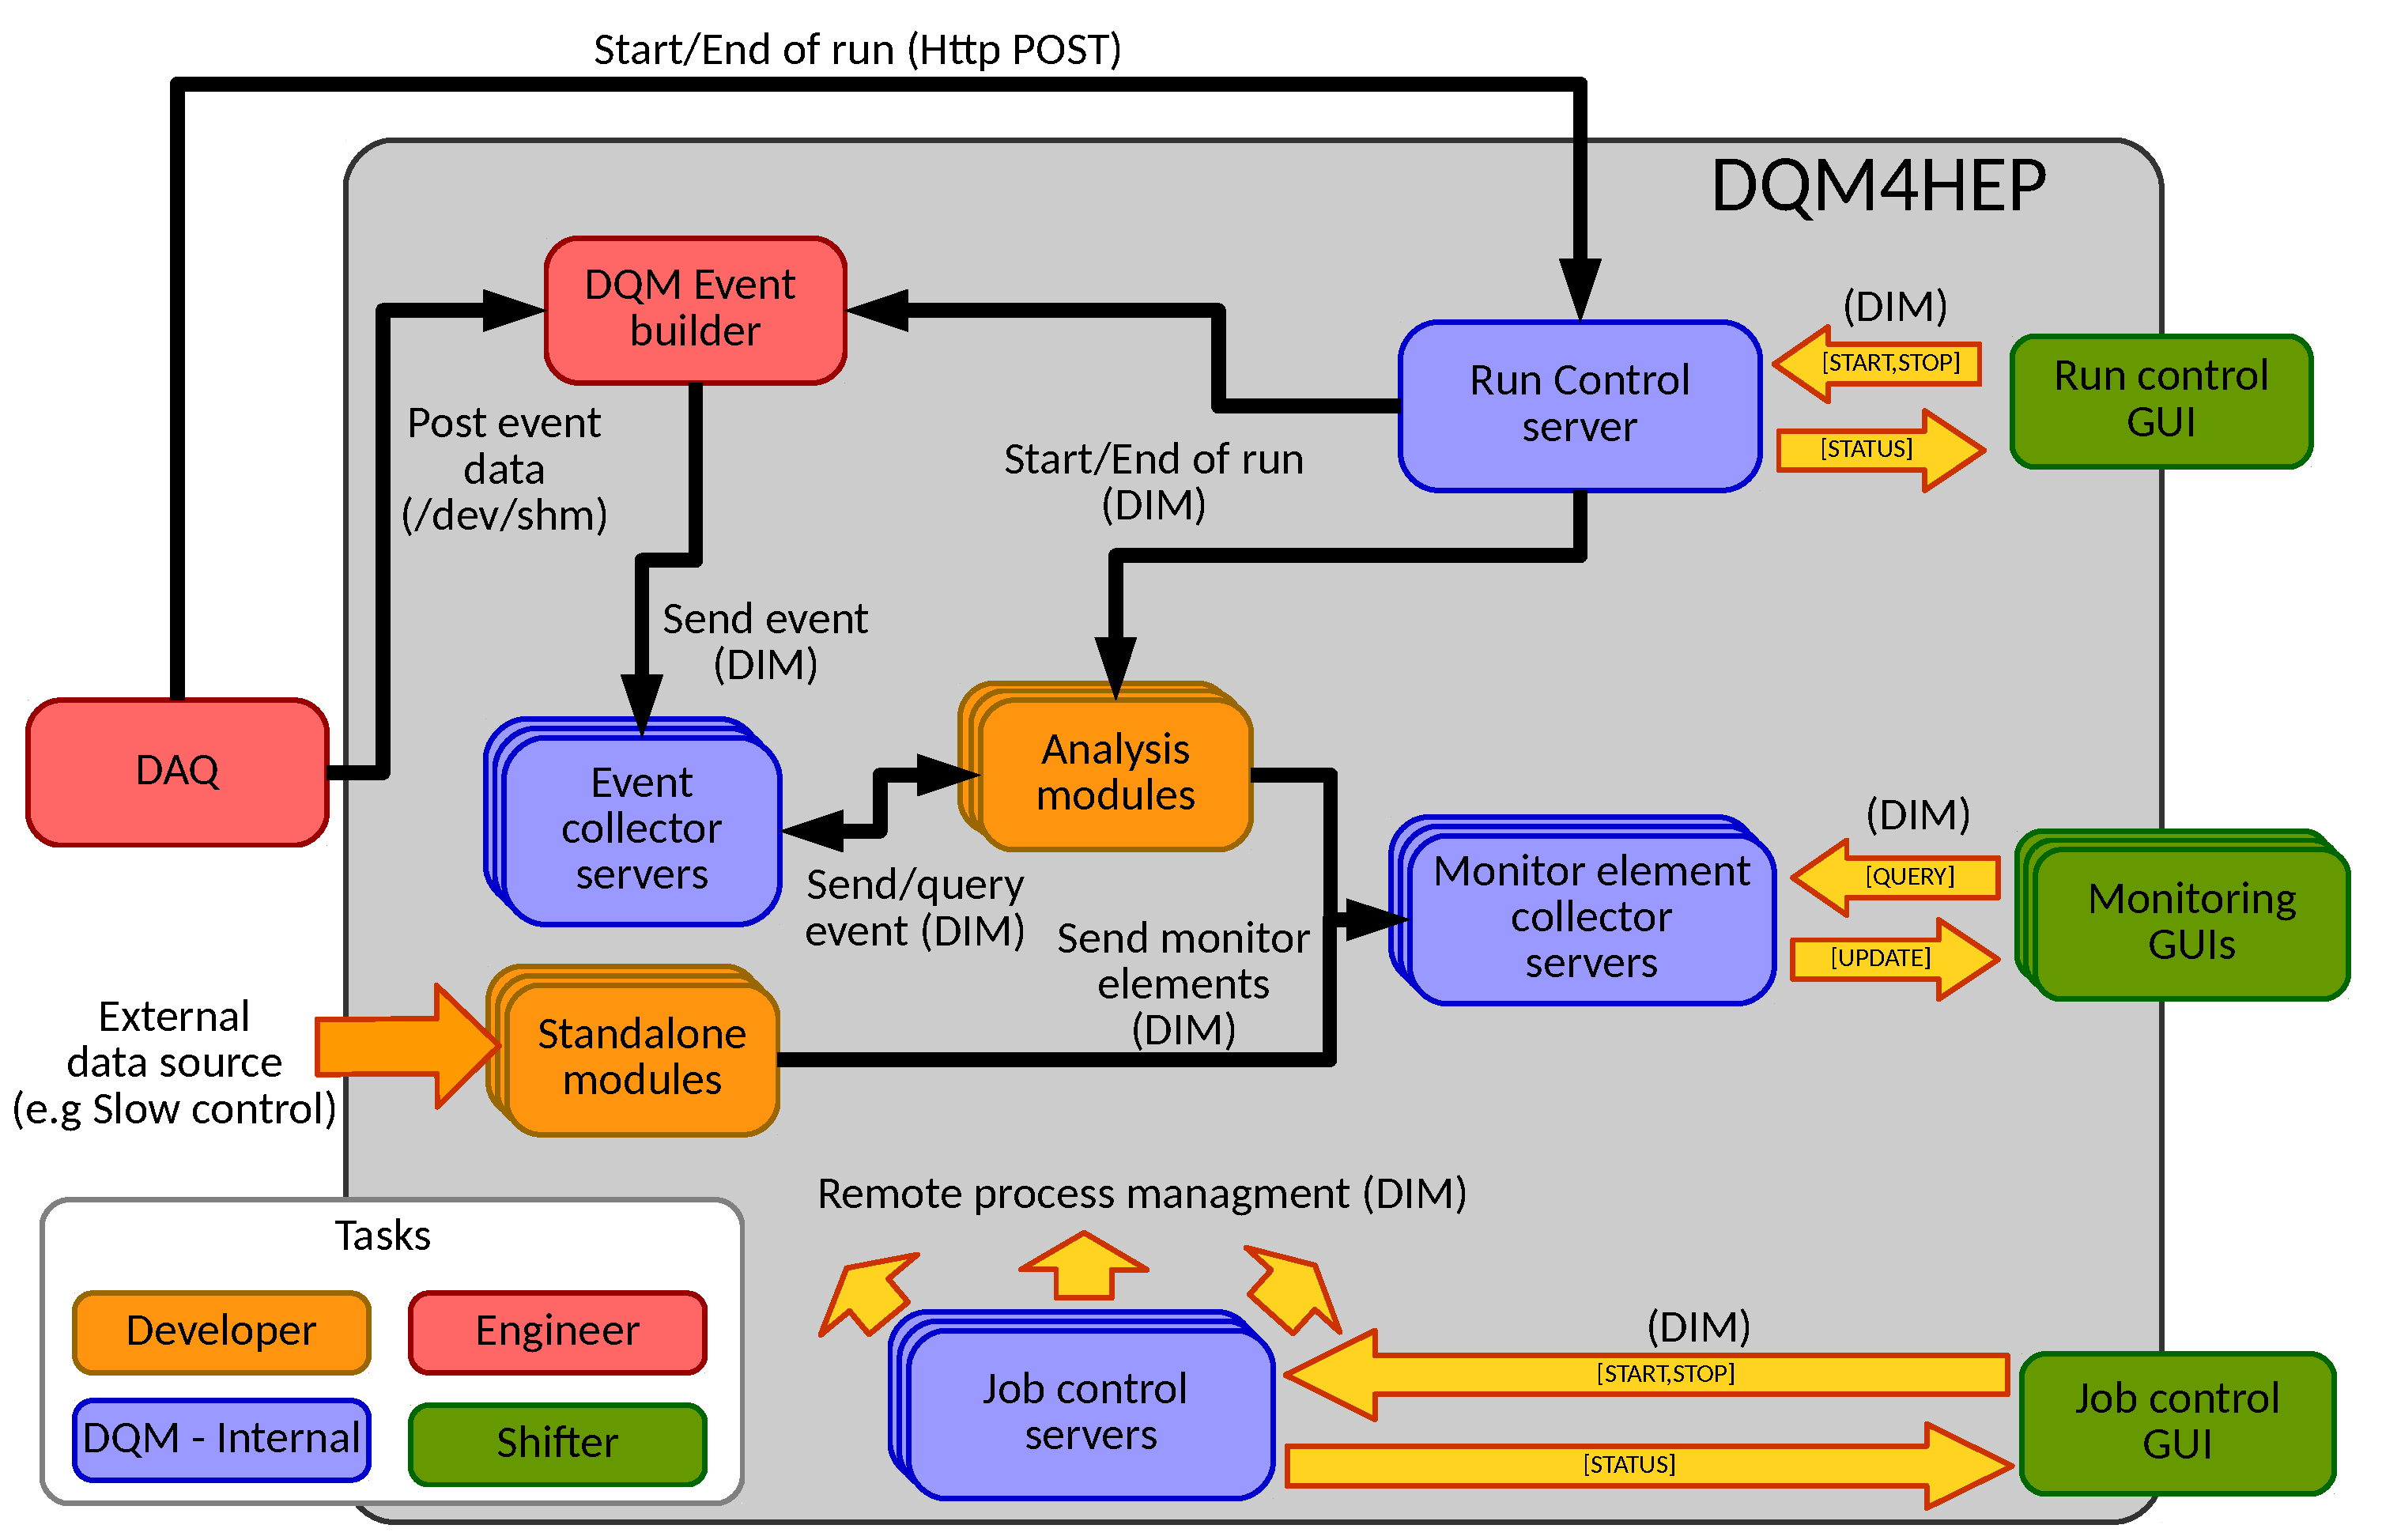
\includegraphics[width=0.9\linewidth]{figs/GlobalArchitectureDiagram.pdf}
\end{frame}

%----------------------------------------------------------------------
\begin{frame}
  \frametitle{DQM4HEP}
  \framesubtitle{Data analysis module}
  \centering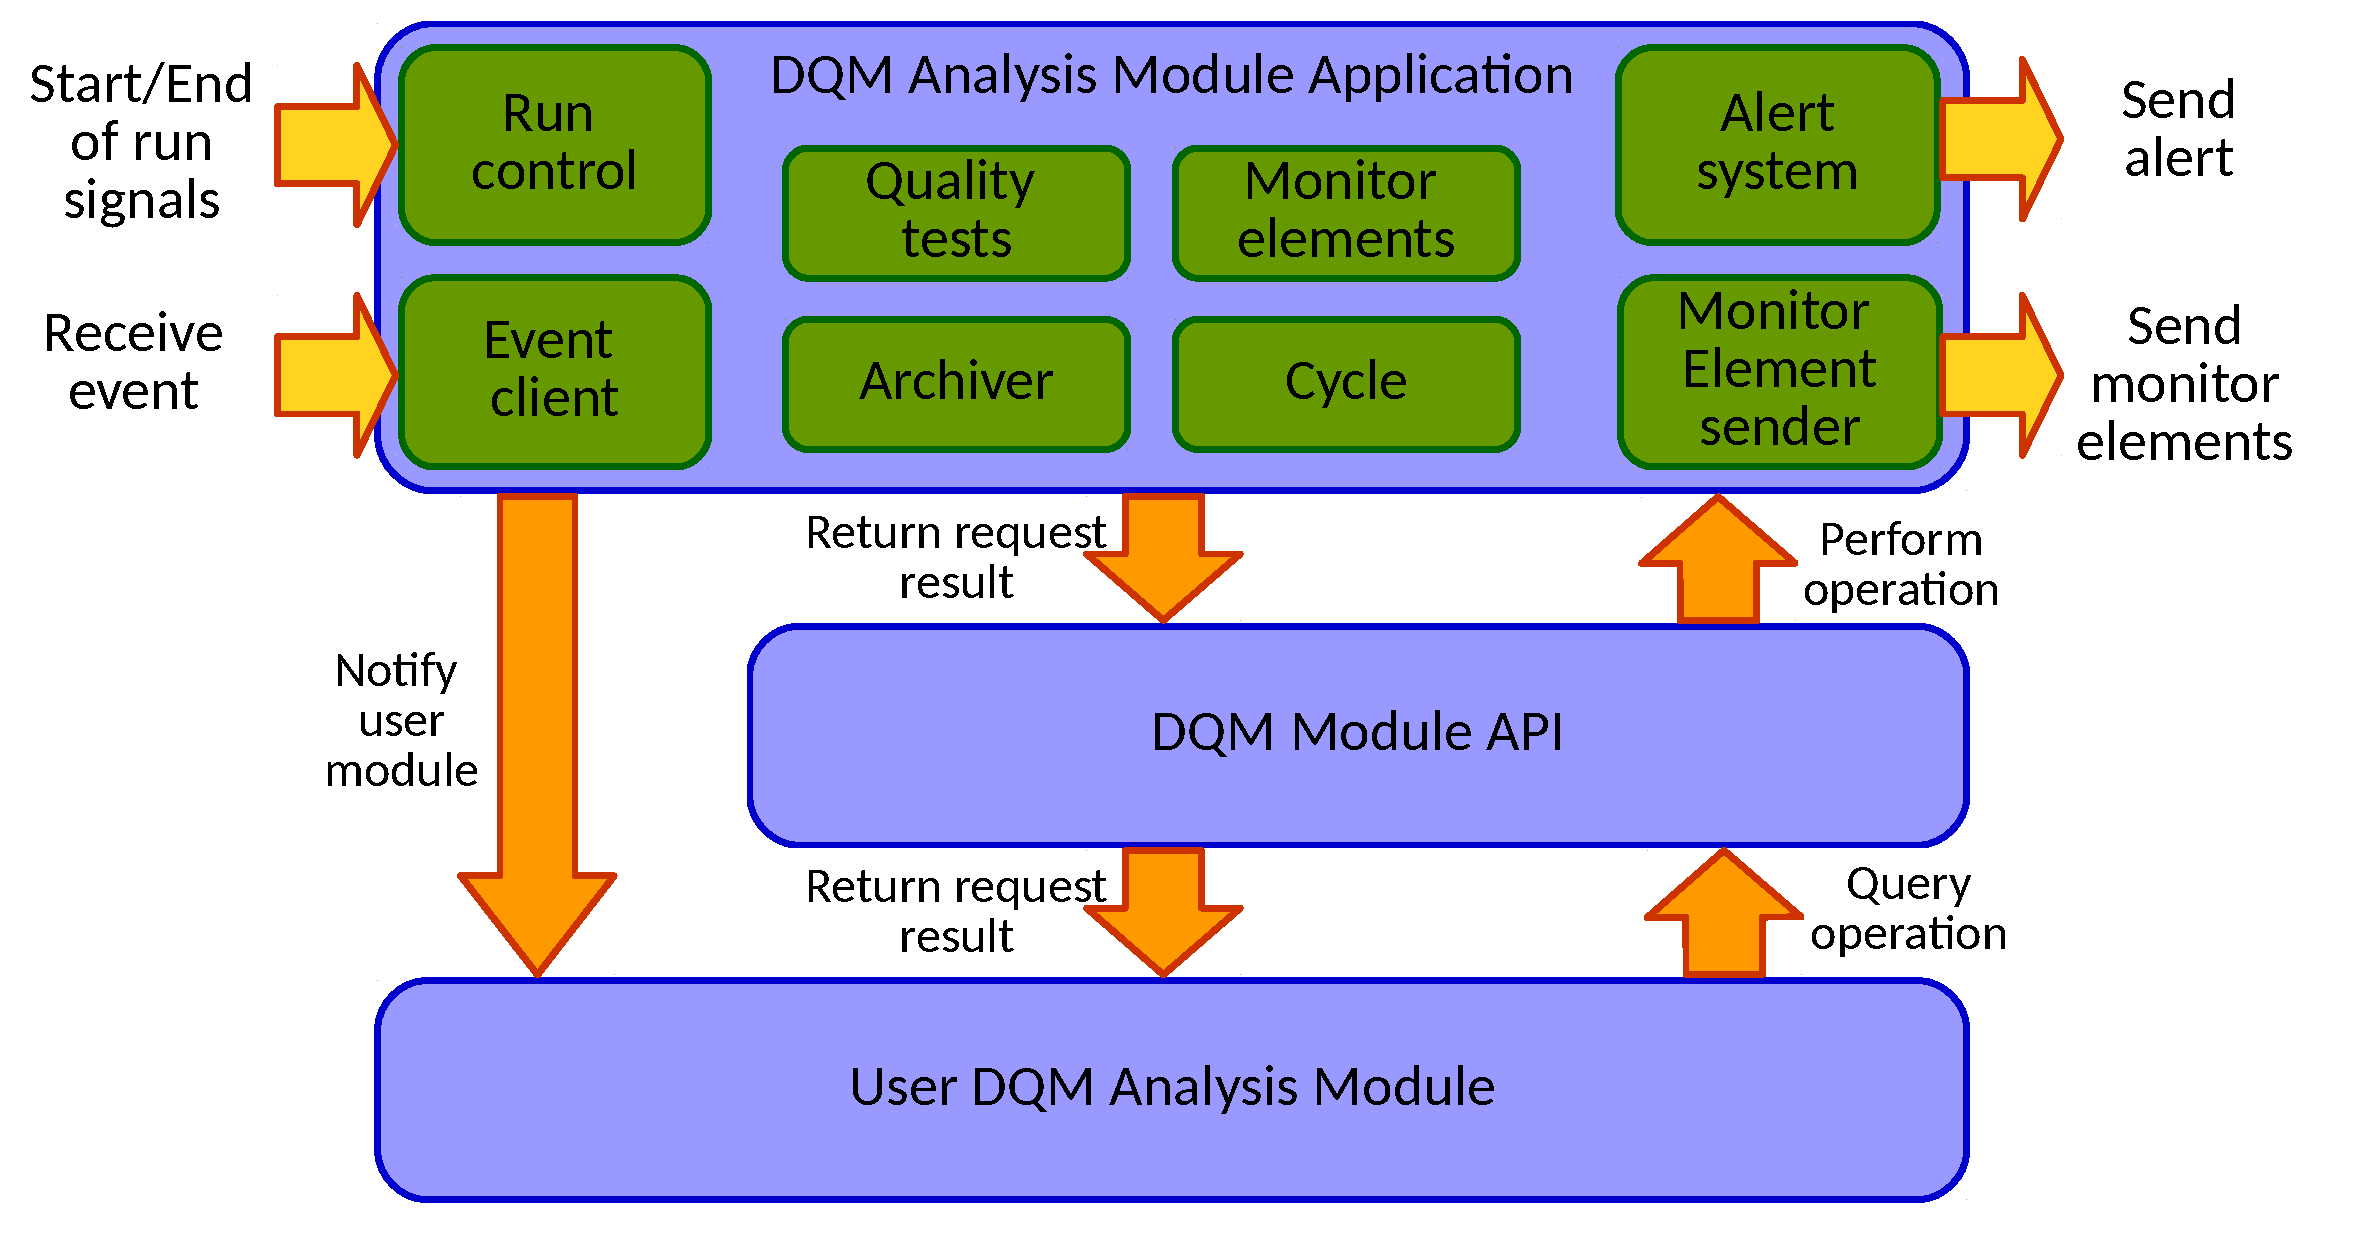
\includegraphics[width=0.9\linewidth]{figs/AnalysisModuleApplicationDiagram.pdf}
\end{frame}

%----------------------------------------------------------------------
\begin{frame}
  \frametitle{DQM4HEP}
  \framesubtitle{Slow control module}
  \centering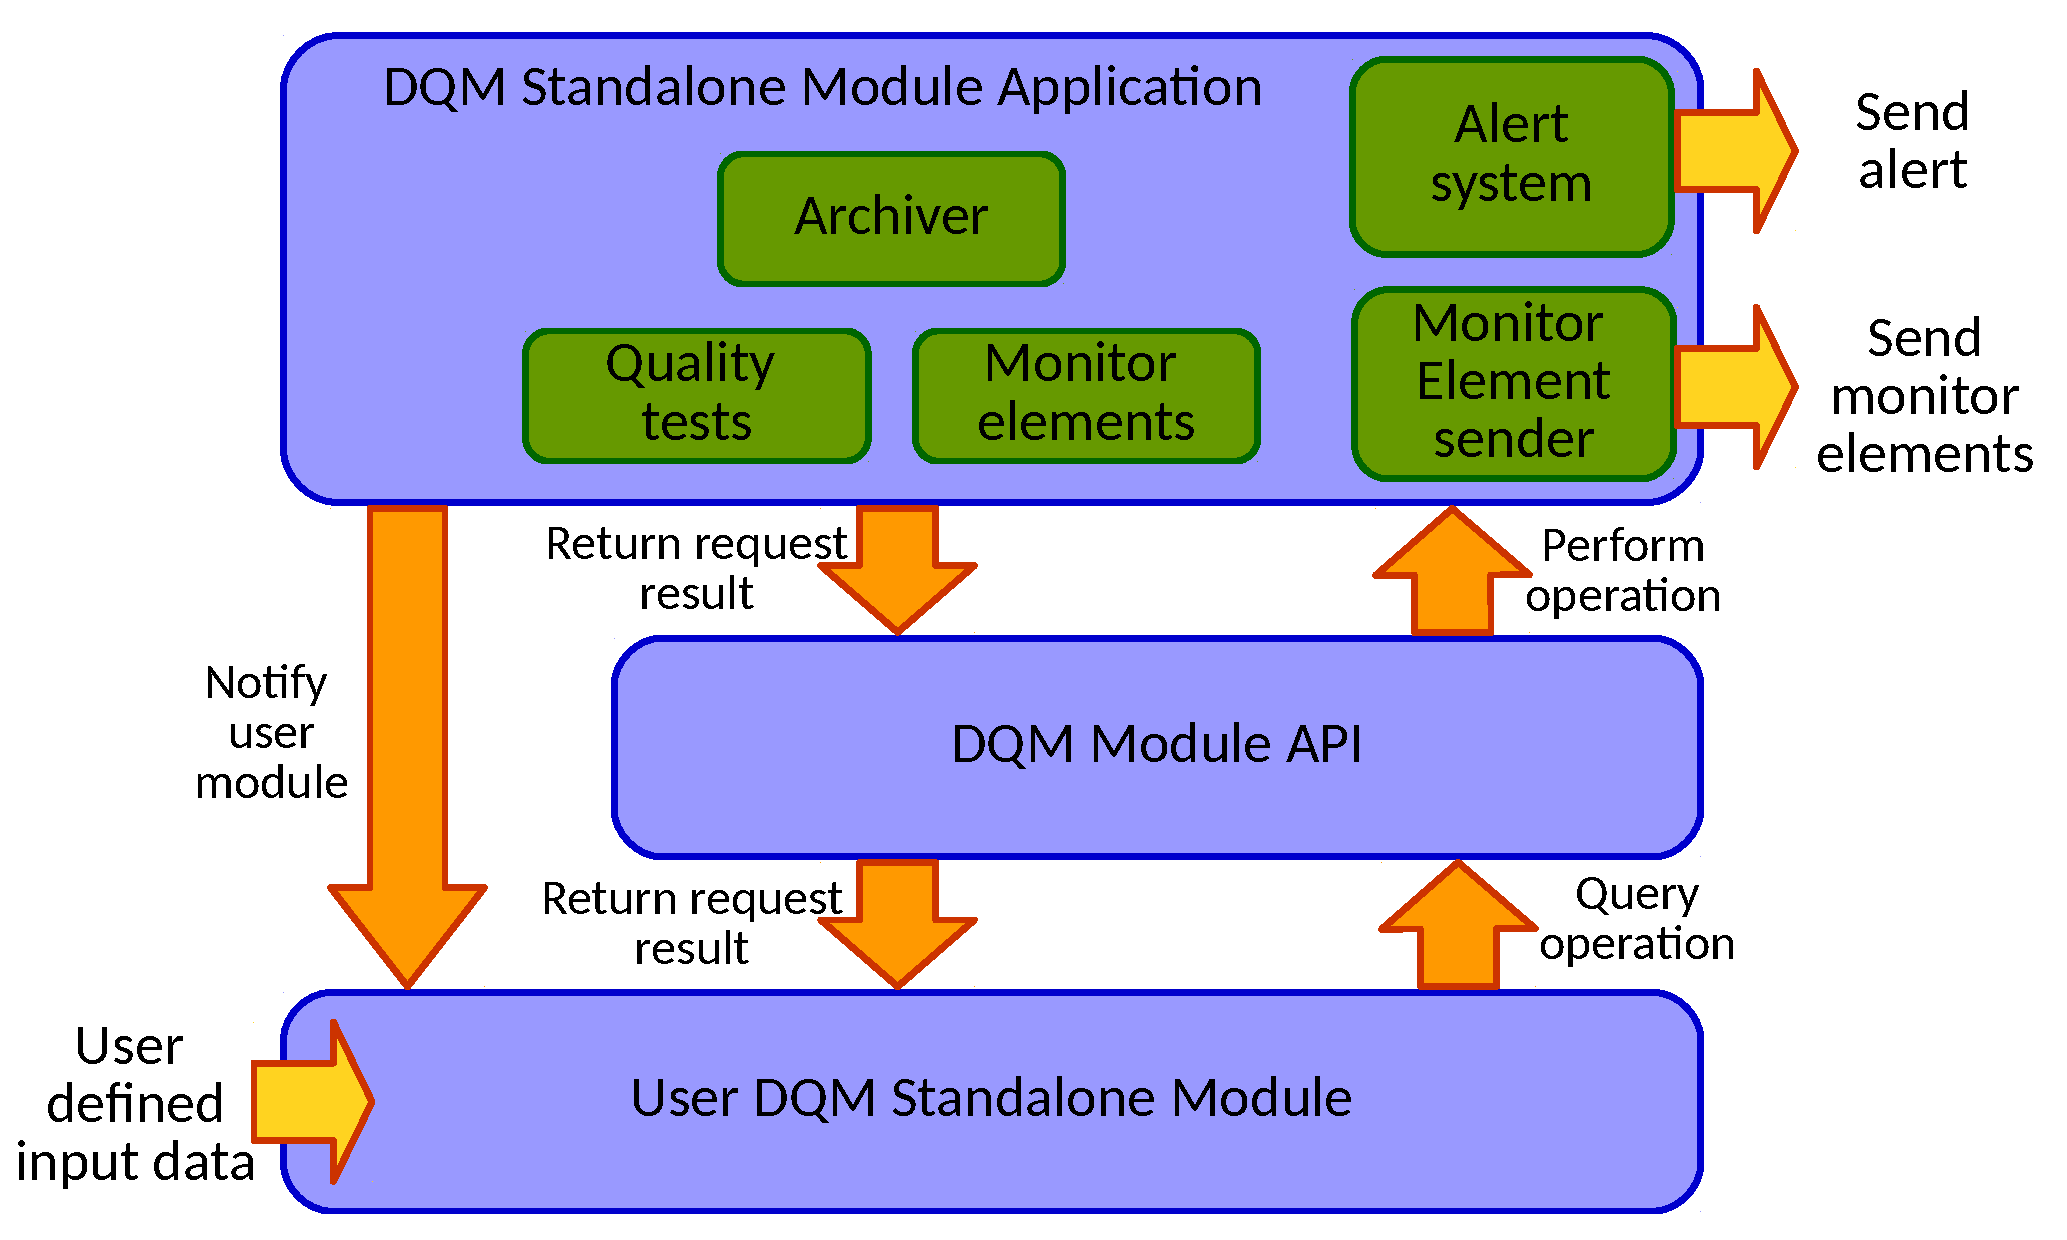
\includegraphics[width=0.9\linewidth]{figs/StandaloneModuleApplicationDiagram.pdf}
\end{frame}

%----------------------------------------------------------------------
\begin{frame}
  \frametitle{DQM4HEP}
  \framesubtitle{Online monitoring interface (Qt Gui)}
    \centering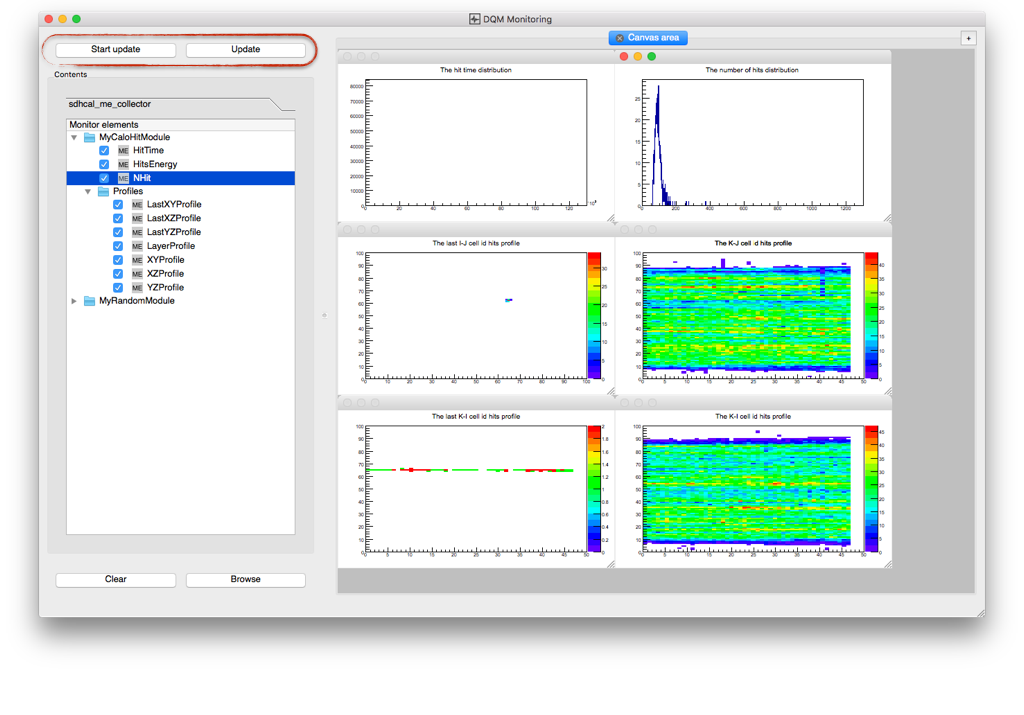
\includegraphics[width=0.95\linewidth]{figs/DQM4HEPMonitoringGui.png}
\end{frame}

%----------------------------------------------------------------------
\begin{frame}
  \frametitle{DQM4HEP}
  \framesubtitle{Detectors using DQM4HEP}
  DQM4HEP used by different detectors in the CALICE collaboration. \\
  ~\\
  
  \begin{minipage}{0.49\linewidth}
    SDHCal online monitoring
    \begin{itemize}
      \item Hit map
      \item Electronics rate
      \item Slow control : I, HV, LW, T, P
      \item GRPC efficiency, multiplicity
    \end{itemize}
    ~\\
    AHCal online monitoring
    \begin{itemize}
      \item Hit map
      \item Correlation with Telescope hits
      \item Electronics rate
    \end{itemize}
  \end{minipage}
  \begin{minipage}{0.49\linewidth}
    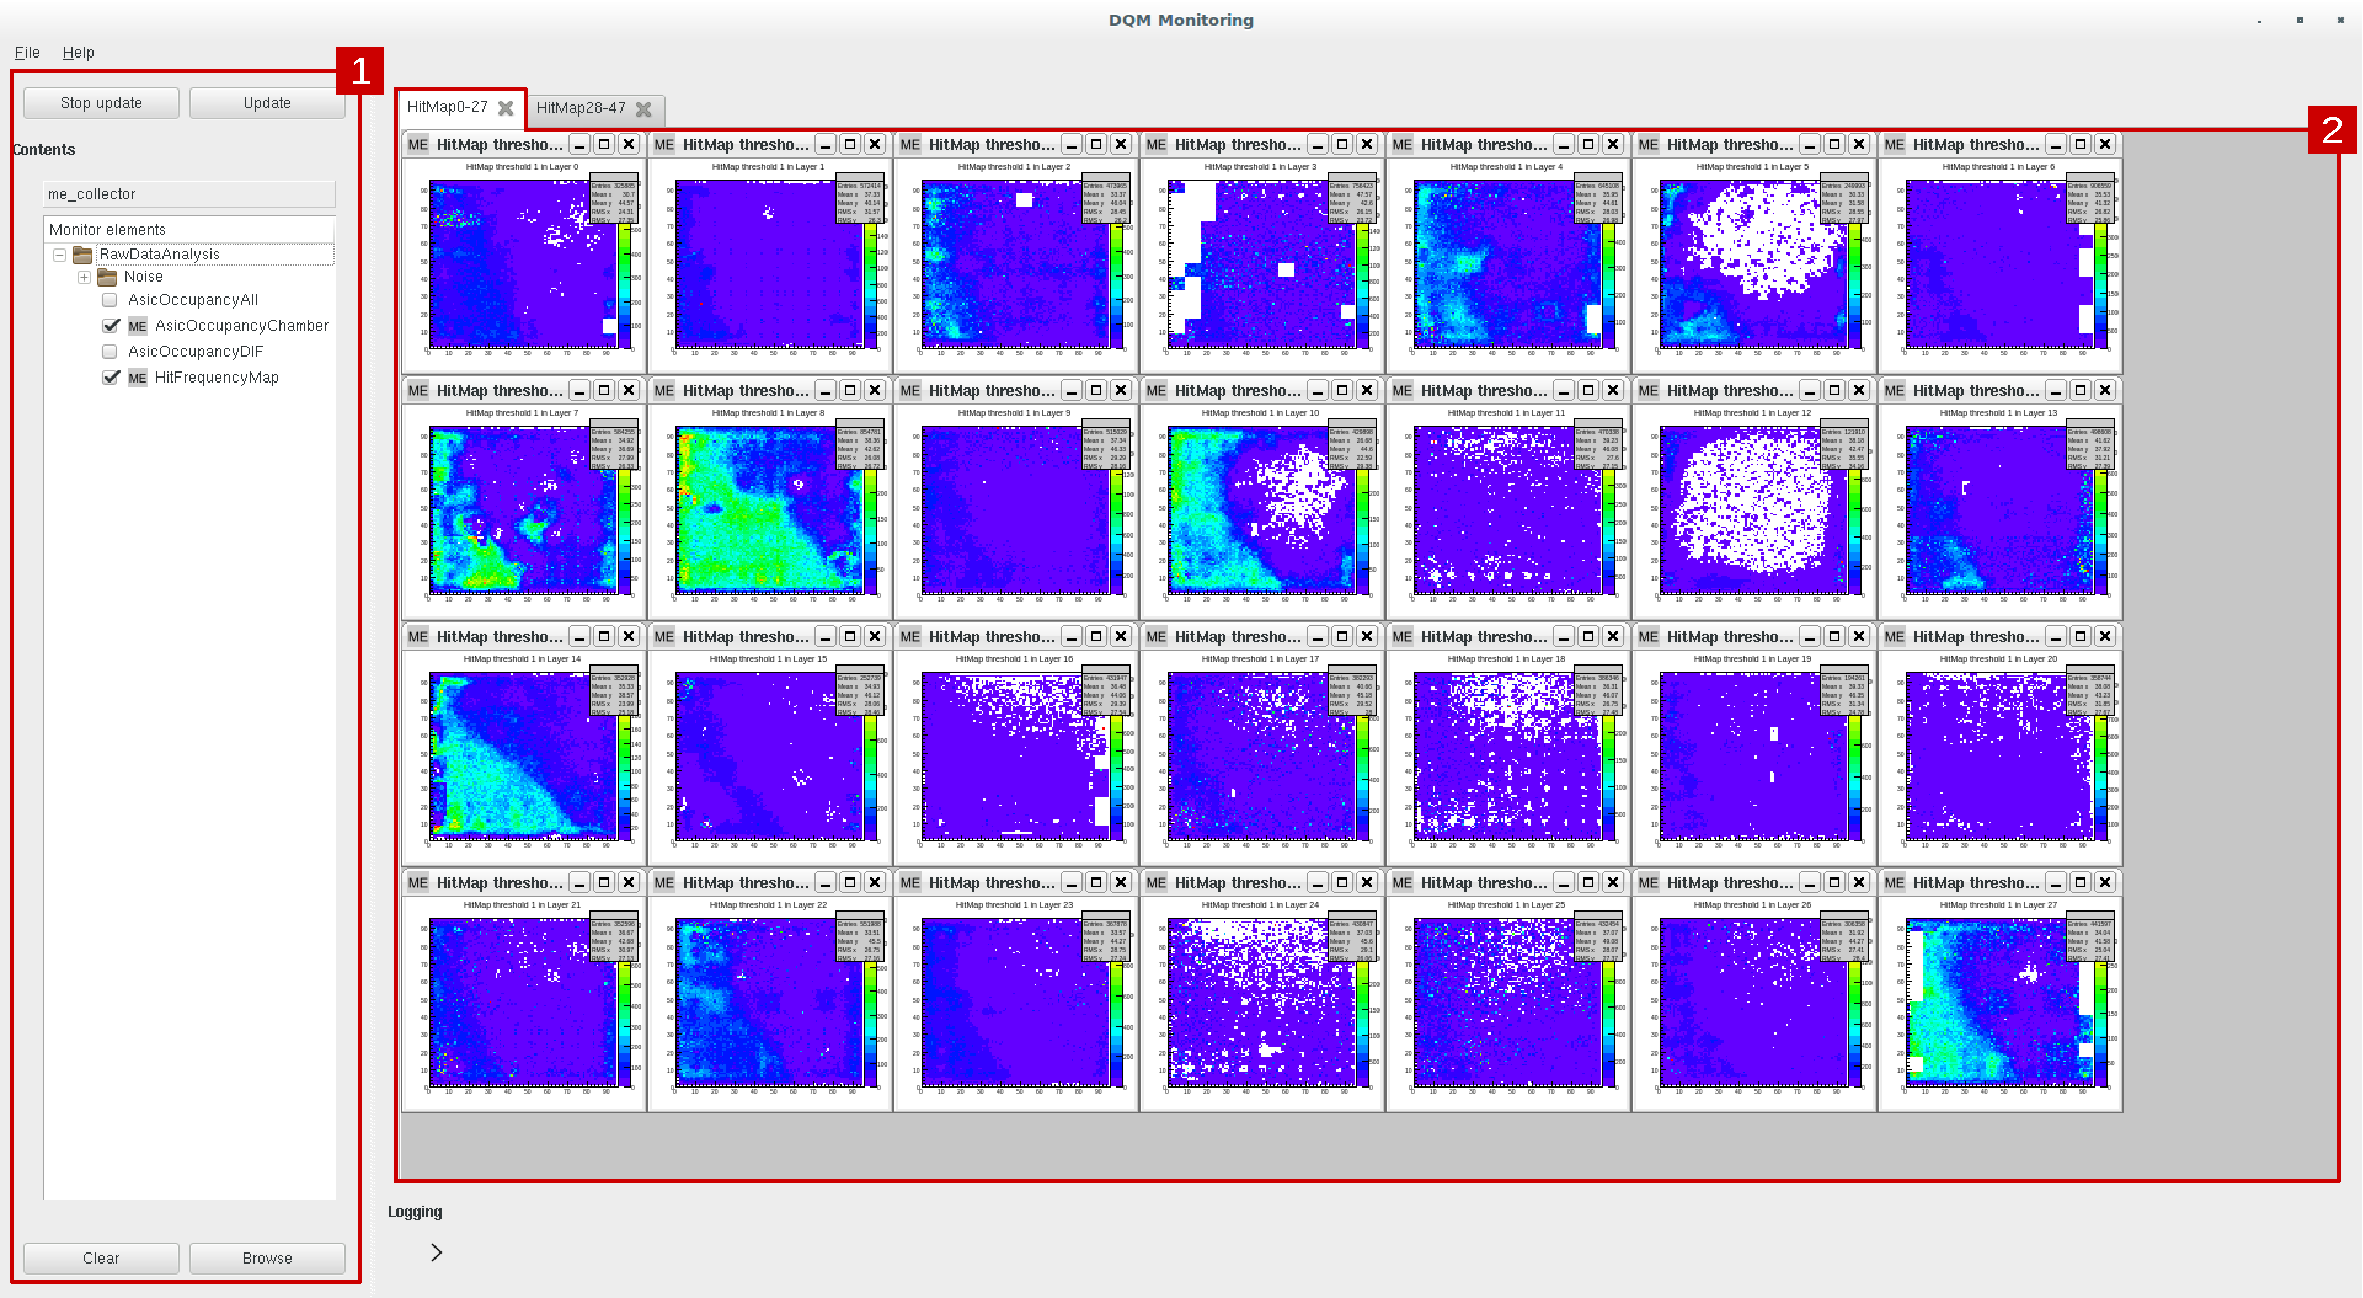
\includegraphics[width=0.95\linewidth]{figs/MonitoringMainWindowGui.pdf} \\
    ~\\
    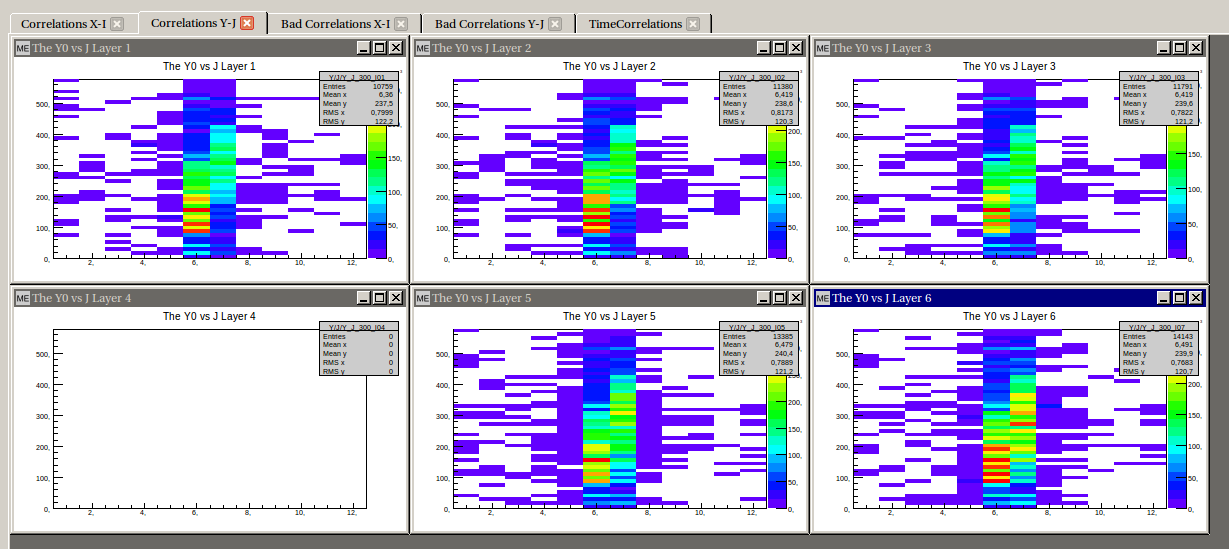
\includegraphics[width=0.95\linewidth]{figs/AHCal_DQM4HEP_CorrelationsYJ.png}
  \end{minipage}
\end{frame}

%----------------------------------------------------------------------
\begin{frame}
  \frametitle{DQM4HEP}
  \framesubtitle{AIDA2020 and EUDAQ binding}
  \scriptsize
  DQM4HEP adopted as monitoring framework by AIDA2020 WP5 :
  \begin{center}
    \fbox{
      \begin{minipage}{0.5\linewidth}
        \begin{center}
          \textit{Task 5.4 Development of data quality \\
          and slow control monitoring}
        \end{center}
      \end{minipage}
    }
  \end{center}
  Binding between the EUDAQ framework and DQM4HEP is ongoing.\\
  ~\\
  Current implementation with EUDAQ is \underline{semi-online} :
  \begin{itemize}
    \item Write EUDAQ event in LCIO format to disk
    \item Read last LCIO events and send to DQM4HEP
  \end{itemize}
  ~\\
  Future integration $\rightarrow$ in the \underline{EUDAQ event builder}
  \begin{itemize}
    \item Replace current EUDAQ monitoring
    \item Send event to DQM4HEP event collector before writing to disk
  \end{itemize}
  ~\\
  Needed work to achieve integration :
  \begin{itemize}
    \item Write EUDAQ event streamer in DQM4HEP framework
    \item Write client interface to EUDAQ run control for SOR/EOR
    \item Final integration in EUDAQ software
  \end{itemize}
\end{frame}


%----------------------------------------------------------------------
\begin{frame}
  \frametitle{DQM4HEP}
  \framesubtitle{Current work (1)}
  \footnotesize
  Next ILC MC production soon (first checks started). \\
  Need for automatic data quality checks for simulated/reconstructed quantities. \\
  ~\\
  Ongoing work to separate the main package (DQMCore) into two pieces :
  \begin{itemize}
    \item \textbf{dqm4hep-core}
    \begin{itemize}
      \item MonitorElement
      \item Quality test
      \item Event interface
      \item Streaming (xdrstream)
      \item Plugin management
      \item DB tools (MySQL)
      \item Logging (spdlog)
    \end{itemize}
    \item \textbf{dqm4hep-online}
    \begin{itemize}
      \item Modules (User classes, Online API)
      \item Event collector (server and client)
      \item Monitor element collector (server and client)
      \item Run control (server, client and external interface)
    \end{itemize}
  \end{itemize}
  
\end{frame}

%----------------------------------------------------------------------
\begin{frame}
  \frametitle{DQM4HEP}
  \framesubtitle{Current work (2)}
  \scriptsize
  Current effort to provide an important set of quality test templates in core library \\
  ~\\
  \begin{minipage}{0.49\linewidth}
    \begin{itemize}
      \item Kolmogorov test (hist + ref)
      \item Mean withing range
      \item Mean 90 within range
      \item No data after limit
      \item No data before limit
      \item Fit function and check chi2
      \item Likelihood fit
      \item Fraction of data after limit exceed
      \item Fraction of data before limit exceed
      \item RMS lower than
      \item RMS 90 lower than
    \end{itemize}
  \end{minipage}
  \begin{minipage}{0.49\linewidth}
    \begin{itemize}
      \item RMS greater than
      \item RMS 90 greater than
      \item Mean lower than
      \item Mean 90 lower than
      \item Mean greater than
      \item Mean 90 greater than
      \item RMS within range
      \item RMS 90 within range
      \item Fit function and check parameters within range
      \item Distance between two values (for scalar comparison)
    \end{itemize}
  \end{minipage} \\
  ~\\
  ~\\
  Incoming work : \textbf{possibility to test any object in any ROOT file with QTests}
\end{frame}

%----------------------------------------------------------------------
\begin{frame}
  \frametitle{DQM4HEP}
  \framesubtitle{URLs and contact}
  GitHub collaboration\\
  \vspace*{0.1cm}
  ~~~
  \begin{minipage}{0.03\linewidth}
    
\includegraphics[width=\linewidth]{figs/github-logo.png}
  \end{minipage}
  \href{https://github.com/dqm4hep}{\tt https://github.com/dqm4hep} \\
  ~\\
  Installation package (\texttt{v04-03-00}) \\
  \vspace*{0.1cm}
  ~~~
  \begin{minipage}{0.03\linewidth}
    
\includegraphics[width=\linewidth]{figs/github-logo.png}
  \end{minipage}
  \href{https://github.com/dqm4hep/dqm4hep}{\tt https://github.com/dqm4hep/dqm4hep} \\
  ~\\
  Slack channel (Announcements, issues, management) \\
  \vspace*{0.1cm}
  ~~~
  \begin{minipage}{0.035\linewidth}
    
\includegraphics[width=\linewidth]{figs/slack-logo.png}
  \end{minipage}
  \href{https://dqm4hep.slack.com}{\tt https://dqm4hep.slack.com} \\
  ~\\
  Contact us !
  \begin{itemize}
    \item R. Ete (\href{mailto:remi.ete@desy.de}{\tt remi.ete@desy.de}) 
    \item A. Pingault (\href{mailto:antoine.pingault@ugent.be}{\tt antoine.pingault@ugent.be})
    \item T. Coates (\href{mailto:tc297@sussex.ac.uk}{\tt tc297@sussex.ac.uk})
  \end{itemize}
  

  % AIDA2020 Milestone report MS67 : \textit{Data quality monitoring tools ready} \\
  % $\rightarrow$ Delivery for end of October 2017 !

\end{frame}




% \begin{itemize}
%   \item Introduction
%   \item Framework presentation
%   \item Experiments running with DQM4HEP
%   \item EUDAQ / DQM4HEP interface
%   \item Current status
%   \item Ongoing and future working
% \end{itemize}

\end{document}

% Enable spell checker for vim
% setlocal spell spelllang=en
